\subsection{Experiment-2. 22.02.2020}\label{experiment-1.-22.02.2020}

The second attempt took place on 22.02.2020.

This time the aim was to test changes in the system components:

\begin{itemize}
	\tightlist
	\item
	A new way to estimate uplink and downlink speed added in \gls{gps_android} using \gls{ftp} (ability to specify IP address for \gls{cnc} in the app)
	\item
	Logging capabilities in \gls{gps_android}
	\item
	Improvements in \gls{gps_frontend} (the uplink/downlink throughput measurements plot, figures became more informative).
\end{itemize}



The goal is to perform an reduced experiment with 1 \gls{command_n_center}, 1 \gls{ap}, and 3 \glspl{ue} with the same settings from the previous experiment but with modified components.

The second \gls{ap} did not participate because of troubles with \gls{wifi} \gls{access_point} installation drivers (later the update to Debian 11 Testing fixed this problem).

\subsection{Weather conditions}

\begin{itemize}
	\tightlist
	\item
	No precipitation
	\item
	Clear sky
	\item
	No snow
	\item
	Strong winds
\end{itemize}

\subsection{Procedure}

Only \hyperref[near-optimal-layout]{Near-Optimal case} was performed.

To exclude possible bottleneck because of additional wireless bearer between \gls{ap} and \gls{command_n_center}, we tried to measure the direct connection to \texttt{cnc} in short distance (shown in Figure \ref{fig:attempt-2-direct-cnc-connection}).

\begin{figure}[H]
	\centering
	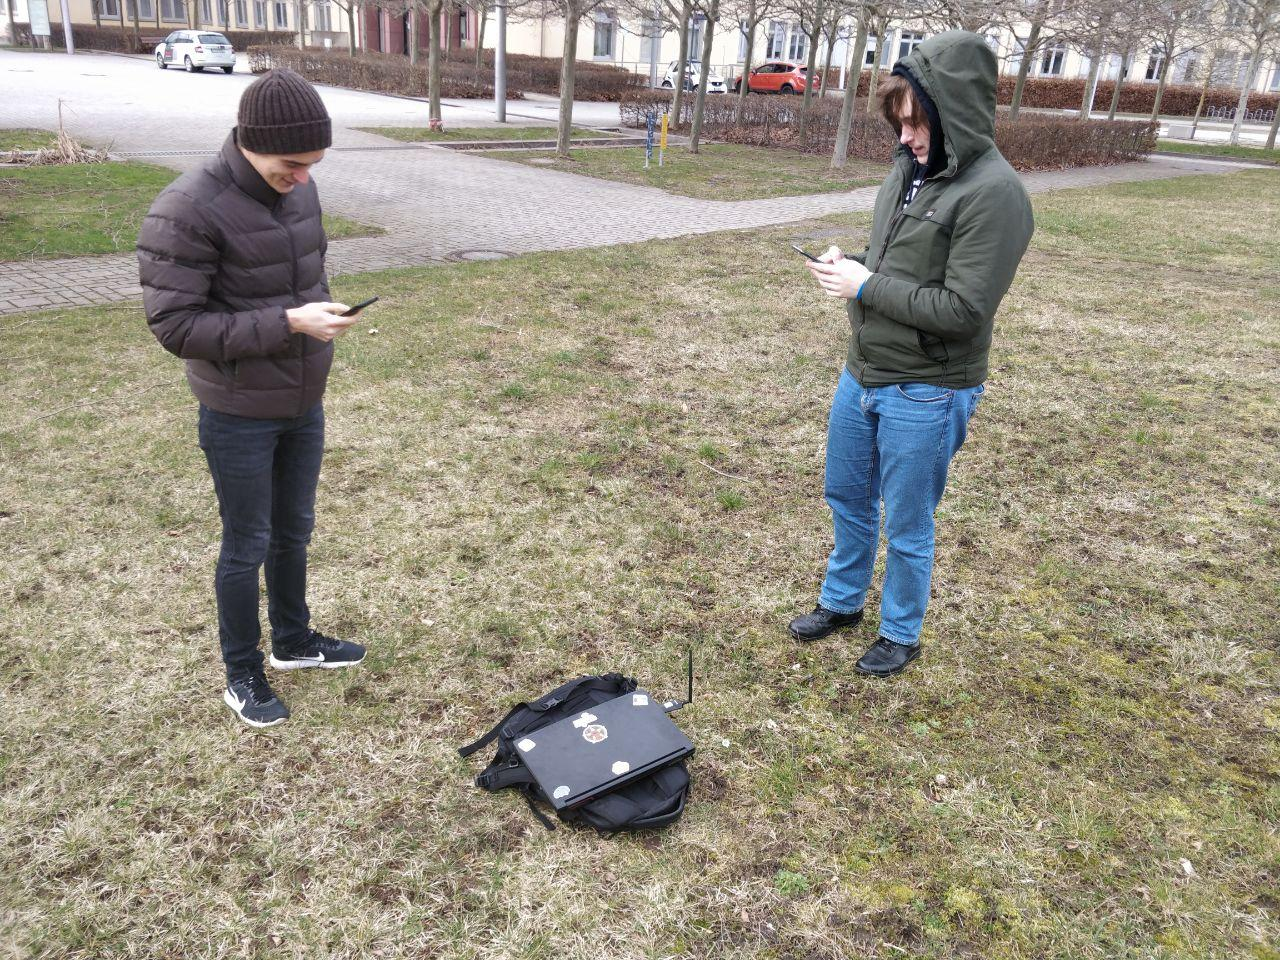
\includegraphics[width=0.7\linewidth,keepaspectratio]{images/experiment_2_overview.jpg}
	\caption{Direct connect to \gls{command_n_center}}
	\label{fig:attempt-2-direct-cnc-connection}
\end{figure}

All \glspl{ue} can connect to \gls{command_n_center} successfully:

\begin{itemize}
	\tightlist
	\item
	deviceId assigned
	\item
	\gls{ue} coordinates displayed
\end{itemize}

During the first half of the experiment, after pressing the `push once' button we received \textbf{uplink/downlink} throughput measurements, however, the values of uplink seemed to be too high \gls{wifi} standard (300 000 kBit/s) compared to downlink (1000-2000 kBit/s).

Later, pressing 'push once' button again did not cause speed re-estimation, the messages from \glspl{ue} did not reach \gls{command_n_center}. The log journal did not contain any error messages. 

\subsection{Outcome}

The second attempt was also not successful. We had not managed to solve the problem in measured data sending. For the next iteration, we proposed to implement some design improvements.

As a result, we decided to:

\begin{itemize}
	\tightlist
	\item
	Add logging capabilities to \glspl{ap}.
	\item
	Implement direct \gls{http} requests and retire \gls{mqtt} broker architecture.
\end{itemize}
